\documentclass[12pt, letter, oneside]{book}
\usepackage{fancyhdr, ifpdf}
\usepackage{float}
\usepackage{setspace}
\usepackage{color}
\usepackage{xcolor}
\usepackage{listings}
\usepackage{caption}
\usepackage[ampersand]{easylist}
\usepackage{amssymb}
\usepackage{pdflscape}
\usepackage{verbatim}
\usepackage{longtable}
\usepackage[margin=1cm]{caption}
\usepackage[top=1in, bottom=.75in, left=.7in, right=1in]{geometry}
\ListProperties(Hide=100, Hang=true, Progressive=3ex,Style*=$\bullet$ , Style2*=-- )

\definecolor{mygray}{rgb}{0.9,0.9,0.9}
\lstdefinestyle{customc}{
  backgroundcolor=\color{mygray},
  captionpos=b, 
  belowcaptionskip=1\baselineskip,
  breaklines=true,
  numbers=left,
  numberstyle=\footnotesize,
  %frame=L,
  xleftmargin=\parindent,
  language=C++,
  showstringspaces=false,
  basicstyle=\footnotesize\ttfamily,
  keywordstyle=\bfseries\color{green!40!black},
  commentstyle=\itshape\color{purple!40!black},
  identifierstyle=\color{black},
  stringstyle=\color{cyan}  
}

\lstset{escapechar=@,style=customc,tabsize=4}

%% some redefination of the headers and footers
\renewcommand{\chaptermark}[1]%
                 {\markboth{#1}{}}
\renewcommand{\sectionmark}[1]%
                 {\markright{\thesection\ #1}}
\lhead[\fancyplain{}{\thepage}]%
      {\fancyplain{}{\rightmark}}
\rhead[\fancyplain{}{\leftmark}]%
      {\fancyplain{}{\thepage}}
\cfoot{}
\sloppy

\ifpdf
   \usepackage[pdftex]{graphicx}
\else
   \usepackage{graphicx}
\fi

\graphicspath{{./Figures/}}
\doublespacing

\begin{document}
\doublespace

\clearpage
\pagenumbering{arabic}

\setcounter{chapter}{0}

\chapter{Add Noise Plugin}
\emph{Add some noise}
\section{Introduction}
The purpose of the \emph{AddNoise} plugin is to introduce random noise to \emph{RoadRunner data}. RoadRunner data is generated internally, and a handle to the underlying data is returned, whenever a user executes RoadRunners \verb|simulate()|, or \verb|simulateEx()| function. 

Generation of actual noise is using the fact that a Rayleigh-distributed random variable $R$, with
the probability distribution $F(R) = 0$ if $R < 0$ and $F(R) = 1 - exp(-R^2/2*\sigma^2)$ if $R >= 0, $
is related to a pair of Gaussian variables $C$ and $D$ through the transformation $C = R * cos(\theta)$ and
$D = R * sin(\theta)$, where $\theta$ is a uniformly distributed variable
in the interval $(0, 2*\pi())$. From Contemporary Communication Systems
USING MATLAB(R), by John G. Proakis and Masoud Salehi, published by
PWS Publishing Company, 1998, pp 49-50. 

 
\section{Plugin Parameters}
In the following, plugin parameters available in the AddNoise plugin are discussed.

\begin{table}[ht]
\centering % used for centering table
\begin{tabular}{l l p{7.5cm}} % centered columns (4 columns)

Parameter Name & Data Type & Purpose \\ [0.5ex] % inserts table 
%heading
\hline % inserts single horizontal line
Sigma         	& 	double & Size of applied noise. \\
NoiseType      	& 	int    & Type of noise generated. Only Gaussian noise is currently supported. \\

\hline %inserts single line
\end{tabular}
\caption{Add noise Plugin Parameters} 
\label{table:AddNoisePluginParameters} 
\end{table}

\section{Plugin Callbacks}
\begin{table}[ht]
\centering % used for centering table
\begin{tabular}{l l p{7.5cm}} % centered columns (4 columns)

Callback & Arguments & Purpose \\ [0.5ex] % inserts table 
%heading
\hline % inserts single horizontal line
PluginStarted  	& 	void*, & Signal to application that the plugin have started applying noise on data. \\
PluginProgress	& 	int*  & Signal progress of noise generation, in \% (0-100\%). \\
PluginFinished	& 	void* & Signal to application the plugin have finished applying noise on data. \\

\hline %inserts single line
\end{tabular}
\caption{AddNoise Plugin callbacks} 
\label{table:AddNoisePluginCallBacks} 
\end{table}

\section{The \texttt{execute()} function}
The AddNoise plugins \verb|execute()| function supports two arguments;

\verb|execute(void* rrData, bool workInThread)|

where \verb|rrData| is a handle to RoadRunner data and \verb|workInThread| is a boolean denoting if the work is to be executed in a thread or not.

\section{Python example}

\begin{singlespace}
\lstinputlisting[label=plugin_addNoise_header,caption={Add noise example.},language=Python]{Examples/rrNoisePlugin.py}
\end{singlespace}

\begin{figure}[H]
\centering
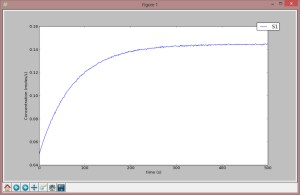
\includegraphics[width=120mm]{AddNoise.jpg}
\caption{Output fot the AddNoise python example script discussed above}
\label{fig:addNoiseFig}
\end{figure}






\end{document}






